\appendix
\section{EconAgent}
\paragraph{Agent Profiles} The initialization of agents' profiles is shown in Figure \ref{fig::age_wage}, including age distribution~(left) and monthly wage distribution~(right), as well as the tax brackets and rates of U.S. federal government in 2018, represented by the gray dotted line. As for the generated jobs aligned with the monthly wage, we show some examples as follows,
\begin{itemize}[leftmargin=*]
    \item \([0, 2454)\): Dog Walker, House Cleaner, Newspaper Delivery \(\ldots\)
    \item \([2454, 4838)\): Barista, Cashier, Fast Food Worker \(\ldots\)
    \item \([35469, 52370)\): Psychiatrist, Pediatrician, Anesthesiologist \(\ldots\)
\end{itemize}

\paragraph{Economic Prompts} We provide a full prompt to illustrate our consideration of economic factors, as well as other details not mentioned in the main text.

\begin{mdframed}[backgroundcolor=gray!20, skipabove=\baselineskip, skipbelow=\baselineskip]
You're Adam Mills, a 40-year-old individual living in New York City, New York. As with all Americans, a portion of your monthly income is taxed by the federal government. This taxation system is tiered, income is taxed cumulatively within defined brackets, combined with a redistributive policy: after collection, the government evenly redistributes the tax revenue back to all citizens, irrespective of their earnings. Now it's 2001.02. In the previous month, you worked as a(an) Professional Athlete. If you continue working this month, your expected income will be \$84144.58, which is decreased compared to the last month due to the deflation of the labor market. Besides, your consumption was \$49825.69. Your tax deduction amounted to \$28216.98. However, as part of the government's redistribution program, you received a credit of \$6351.29. In this month, the government sets the brackets: [0.00, 808.33, 3289.58, 7016.67, 13393.75, 17008.33, 42525.00] and their corresponding rates: [0.10, 0.12, 0.22, 0.24, 0.32, 0.35, 0.37]. Income earned within each bracket is taxed only at that bracket's rate. Meanwhile, deflation has led to a price decrease in the consumption market, with the average price of essential goods now at \$135.82. Your current savings account balance is \$12456.42. Interest rates, as set by your bank, stand at 3.00\%. With all these factors in play, and considering aspects like your living costs, any future aspirations, and the broader economic trends, how is your willingness to work this month? Furthermore, how would you plan your expenditures on essential goods, keeping in mind goods price? Please share your decisions in a JSON format. The format should have two keys: 'work' (a value between 0 and 1 with intervals of 0.02, indicating the willingness or propensity to work) and 'consumption' (a value between 0 and 1 with intervals of 0.02, indicating the proportion of all your savings and income you intend to spend on essential goods).
\end{mdframed}



\begin{figure}[h]
\centering
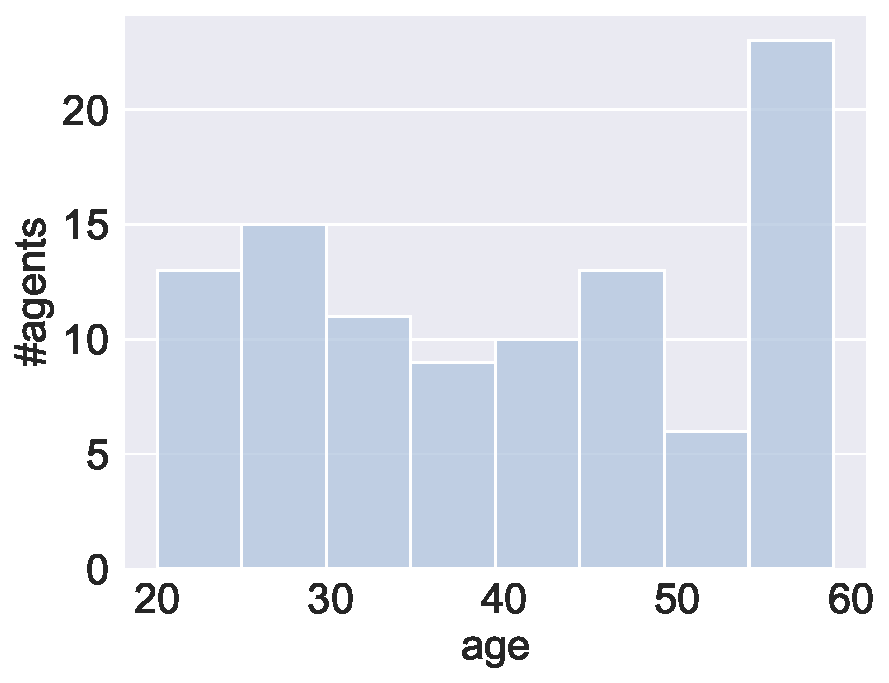
\includegraphics[width=0.44\columnwidth]{figs/age.pdf}
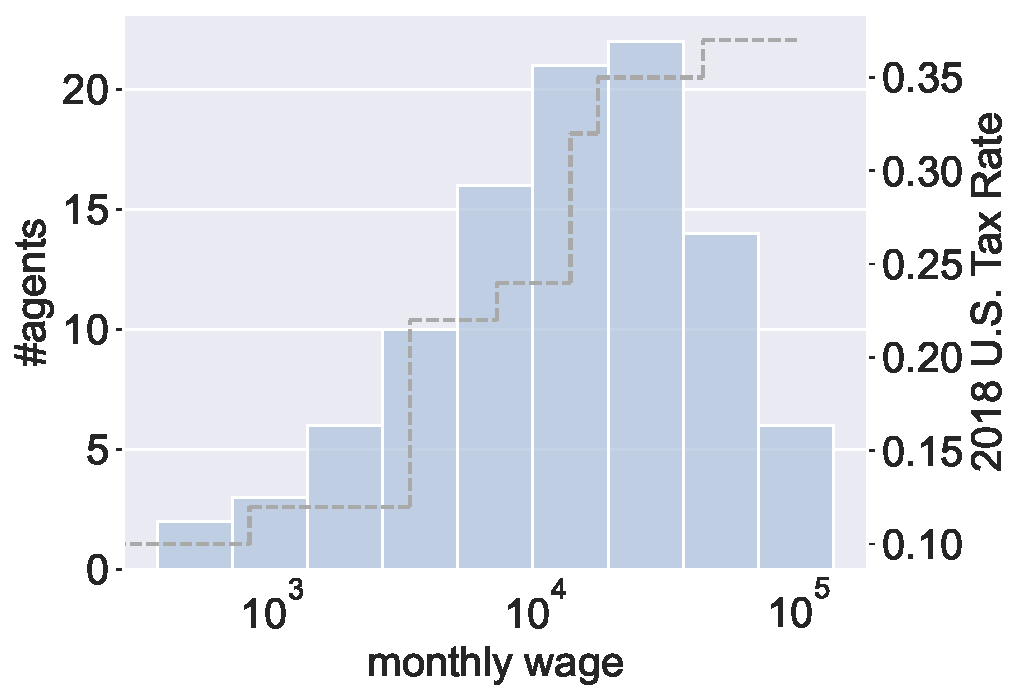
\includegraphics[width=0.49\columnwidth]{figs/wage.pdf}
\caption{Age and monthly wage distribution for agent profiles.} \label{fig::age_wage}
\end{figure}

\section{Experimental Setup}
\paragraph{Baselines}
\begin{itemize}[leftmargin=*]
    \item \textbf{Consumption}. In LEN, the consumption decision is \textit{memory-based}, which means that consumption is influenced not only by current income but also by past accumulated savings. Besides, the goods price is another important factor. Conversely, in CATS, it is \textit{non-memory-based} consumption decisions suggesting that consumption is solely related to the current income. The agent aims to keep a desired ratio between savings and income, and consumption is only a proportion of the income. For more human-like decisions, we also introduce the influence of interest rate in the decision rule.

    For LEN, the calculation of consumption propensity is as follows,
    \begin{equation}
        p_i^c = \left(\frac{P}{s_i+z_i}\right)^{\beta}, \beta\in [0, 1].
    \end{equation}
    For CATS, the calculation is as follows,
    \textit{i.e.},
    \begin{equation}
        \frac{\hat{s}_i}{z_i} = \frac{(1+r)(s_i + (1-c)z_i)}{z_i} = h, p_i^c = \frac{c z_i}{s_i + z_i},
    \end{equation}
    where $\hat{s}_i$ denotes the expected savings after consumption in the next month, $h$ is a constant, and $c$ indicates the consumption proportion of the current income. Refer to CATS for the calculation of $c$. Note that we introduce the influence of the interest rate $r$ to endow the agent with the perception of fiscal policy.

    \item \textbf{Work}. The rule of working in LEN and CATS can not be directly used in our simulation framework because we don't simulate firms. Therefore, we follow the intuitions of their designs and define a formula implying that a higher expected income, lower savings, or a lower interest rate leads to a greater propensity to work.

    The work propensity is calculated as
    \begin{equation}
        p^w_i = \left(\frac{v_i}{s_i(1+r)}\right)^{\gamma}, \gamma\in [0, 1].
    \end{equation}

\end{itemize}

For AI-Economist, the utility is a satisfaction function positively correlated with savings and consumption but negatively correlated with labor. Maximizing utility implies that the agent always desires more savings and consumption but prefers less labor. The policy network for the agent's work and consumption decisions is a multi-layer perceptron~(MLP), where the input includes various environment information, such as monthly wage, interest rate, goods price, tax rates, \textit{etc}. We modify the utility function to incorporate consumption and goods price, defined as
\begin{equation}
    \frac{(s_i/P)^{1-\lambda_s}-1}{1-\lambda_s}\cdot \frac{(\hat{c}_i/P)^{1-\lambda_c}-1}{1-\lambda_c} - \lambda_l l_i,
\end{equation}
where $\lambda_{s,c,l}$ balance the importance of savings, consumption, and labor contributing to agent satisfaction. Besides, it's discouraged to not work or have no consumption at all, which leads to negative utility. We also introduce the goods price to make the AI agent perceive the dynamics of the consumption market.

\paragraph{Simulation Parameters} For LEN, CATS, and Composite, we conduct a careful grid search for proper hyperparameters $\beta, \gamma, h$ in decision rules, with the search spaces of $[0.05, 0.1, 0.3, 0.5], [0.05, 0.1, 0.3, 0.5]$, $[0.5, 1, 3, 5]$, respectively. The reported results in the main text are obtained with $\beta=0.1, \gamma=0.1, h=1$, which show the most reasonable macroeconomic indicators.

\paragraph{LLM Costs} Each simulation based on EconAgent incurs a cost of approximately \$30 and takes about 2 hours to complete.

\section{Additional Results} 

\paragraph{Quaterly Indicators} Figure~\ref{fig::quarter-indicators} presents quarterly macroeconomic indicators, where the conclusion is similar to that of annual ones. For AI-Economist, we follow ~\cite{zheng2022ai} to adopt PPO algorithm~\cite{schulman2017proximal} to train the policy network, where the actor and critic networks have the hidden dimensions of $[128, 128]$ and $[128, 64, 32]$, respectively. The observation~(input) dimension is 173 and the action~(output) dimension is 53, including 2 work actions and 51 consumption actions~(0-1 with an interval of 0.02). The training process is shown in Figure \ref{fig::ai}, including the loss and average episode reward, where one episode is a complete simulation of 20 years.

\begin{figure}[t]
\centering
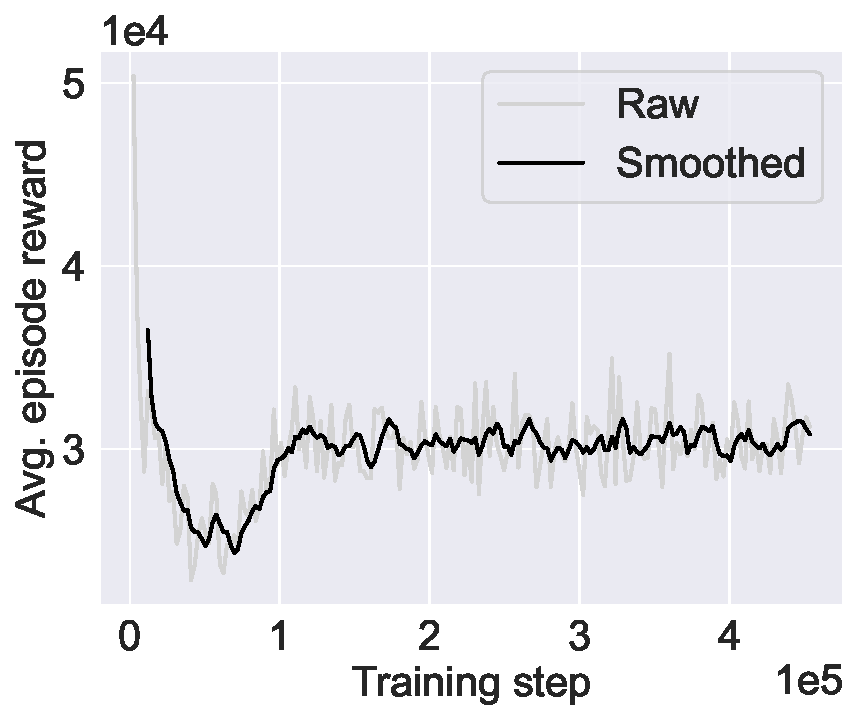
\includegraphics[width=0.44\columnwidth]{figs/mlp_reward.pdf}
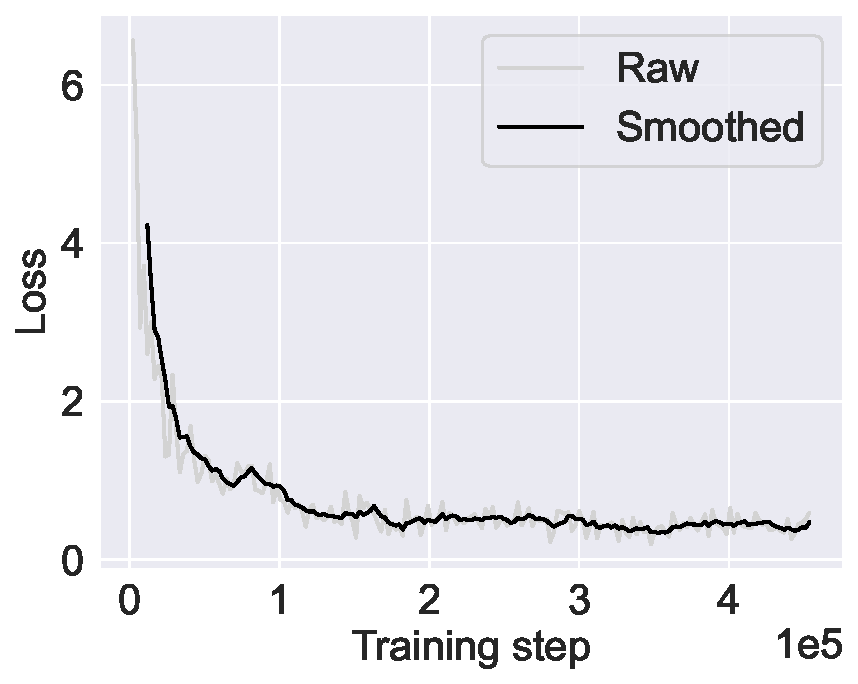
\includegraphics[width=0.44\columnwidth]{figs/mlp_loss.pdf}
\caption{The training process of AI-Economist.} \label{fig::ai}
\end{figure}



\begin{figure}[h!]
\centering

\includegraphics[width=0.9\linewidth]{figs/legend-line.pdf} \
\subfloat{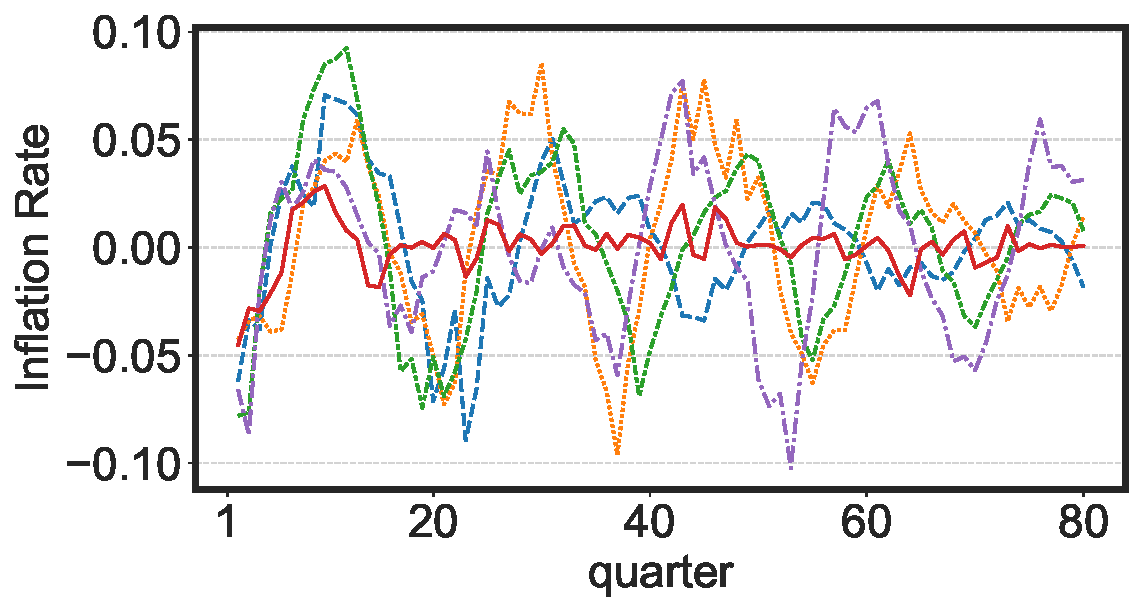
\includegraphics[width=0.9\linewidth]{figs/inflation-quarter.pdf}} \
\subfloat{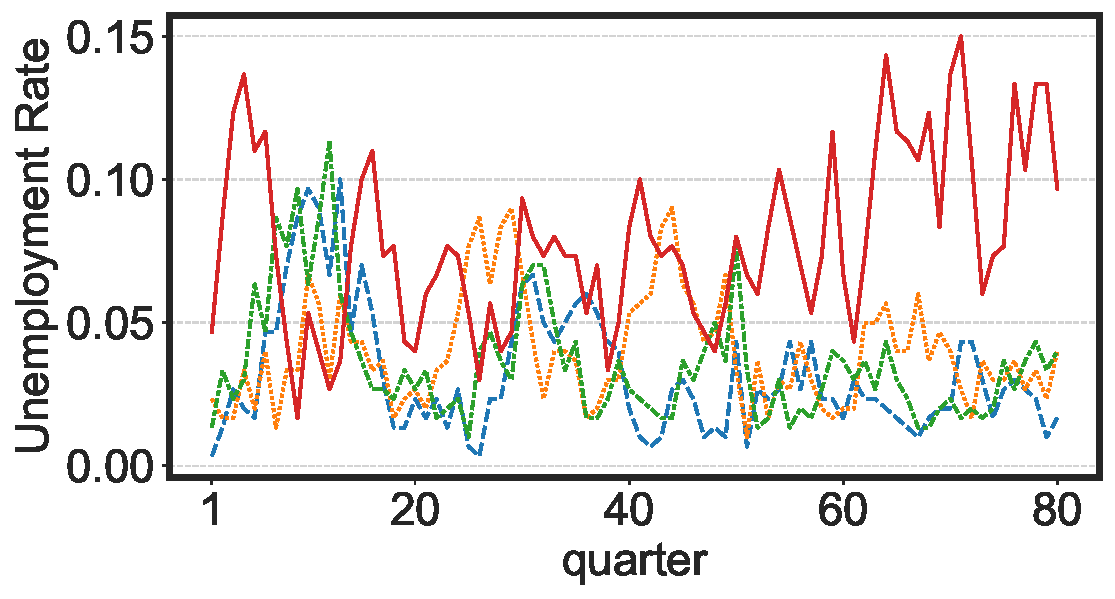
\includegraphics[width=0.9\linewidth]{figs/unemployment-quarter.pdf}} \
\subfloat{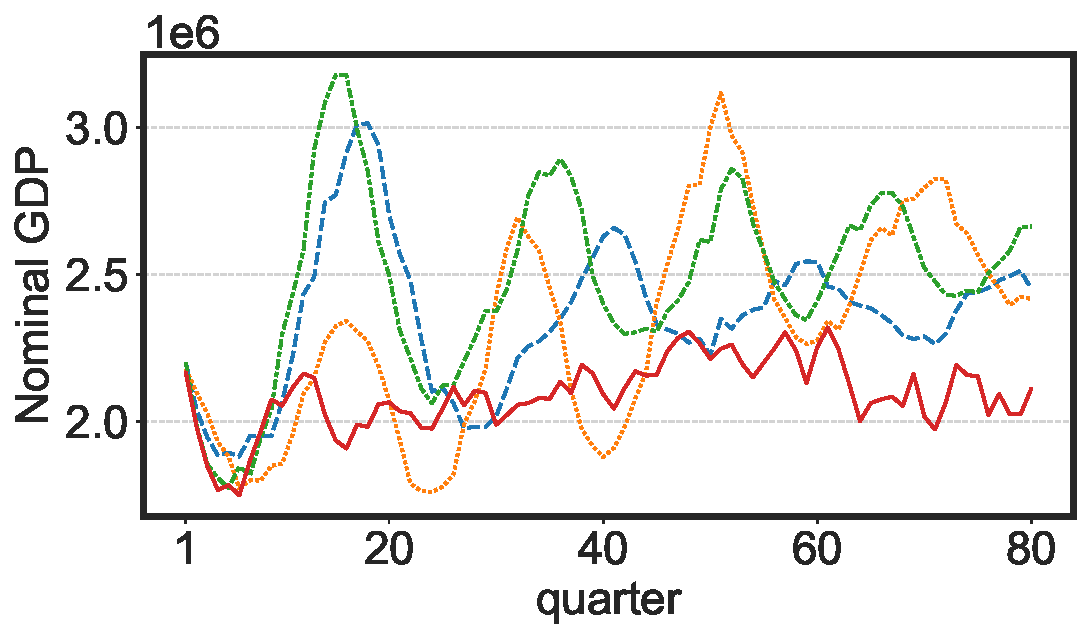
\includegraphics[width=0.9\linewidth]{figs/nominal_gdp-quarter.pdf}} \
\subfloat{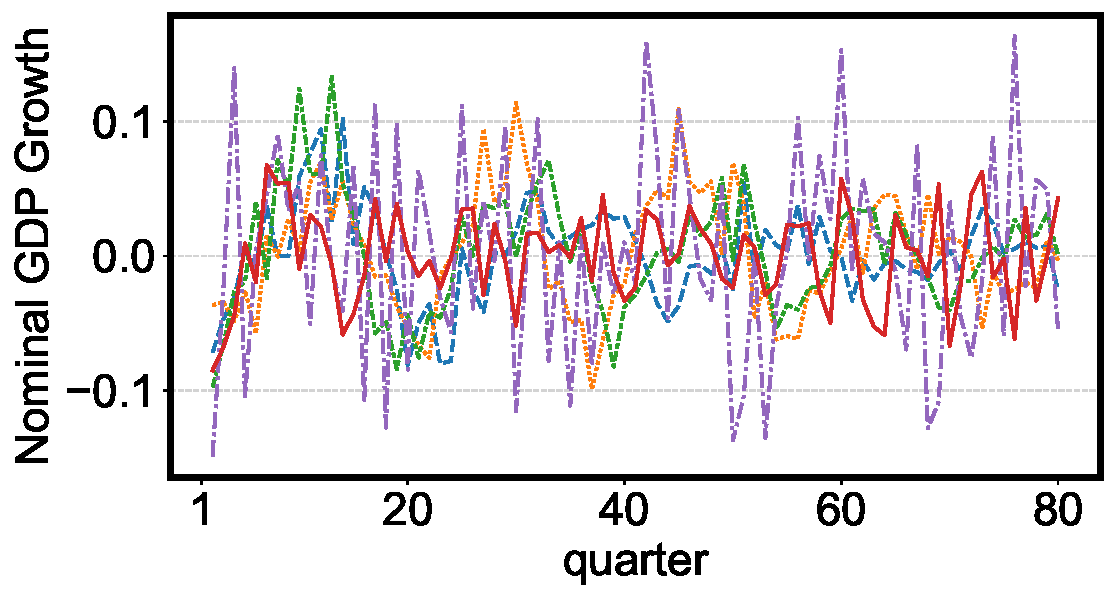
\includegraphics[width=0.9\linewidth]{figs/nominal_gdp_growth-quarter.pdf}} \
\caption{Quarterly variations of macroeconomic indicators.}\label{fig::quarter-indicators}
\end{figure}

\paragraph{Fluctuated Unemployment Rate} The unemployment rate after $5$ additional years of simulation is shown in Figure \ref{fig::unemployment-c}, which returns to a lower level after the 20th year.

\begin{figure}[h!]
\centering
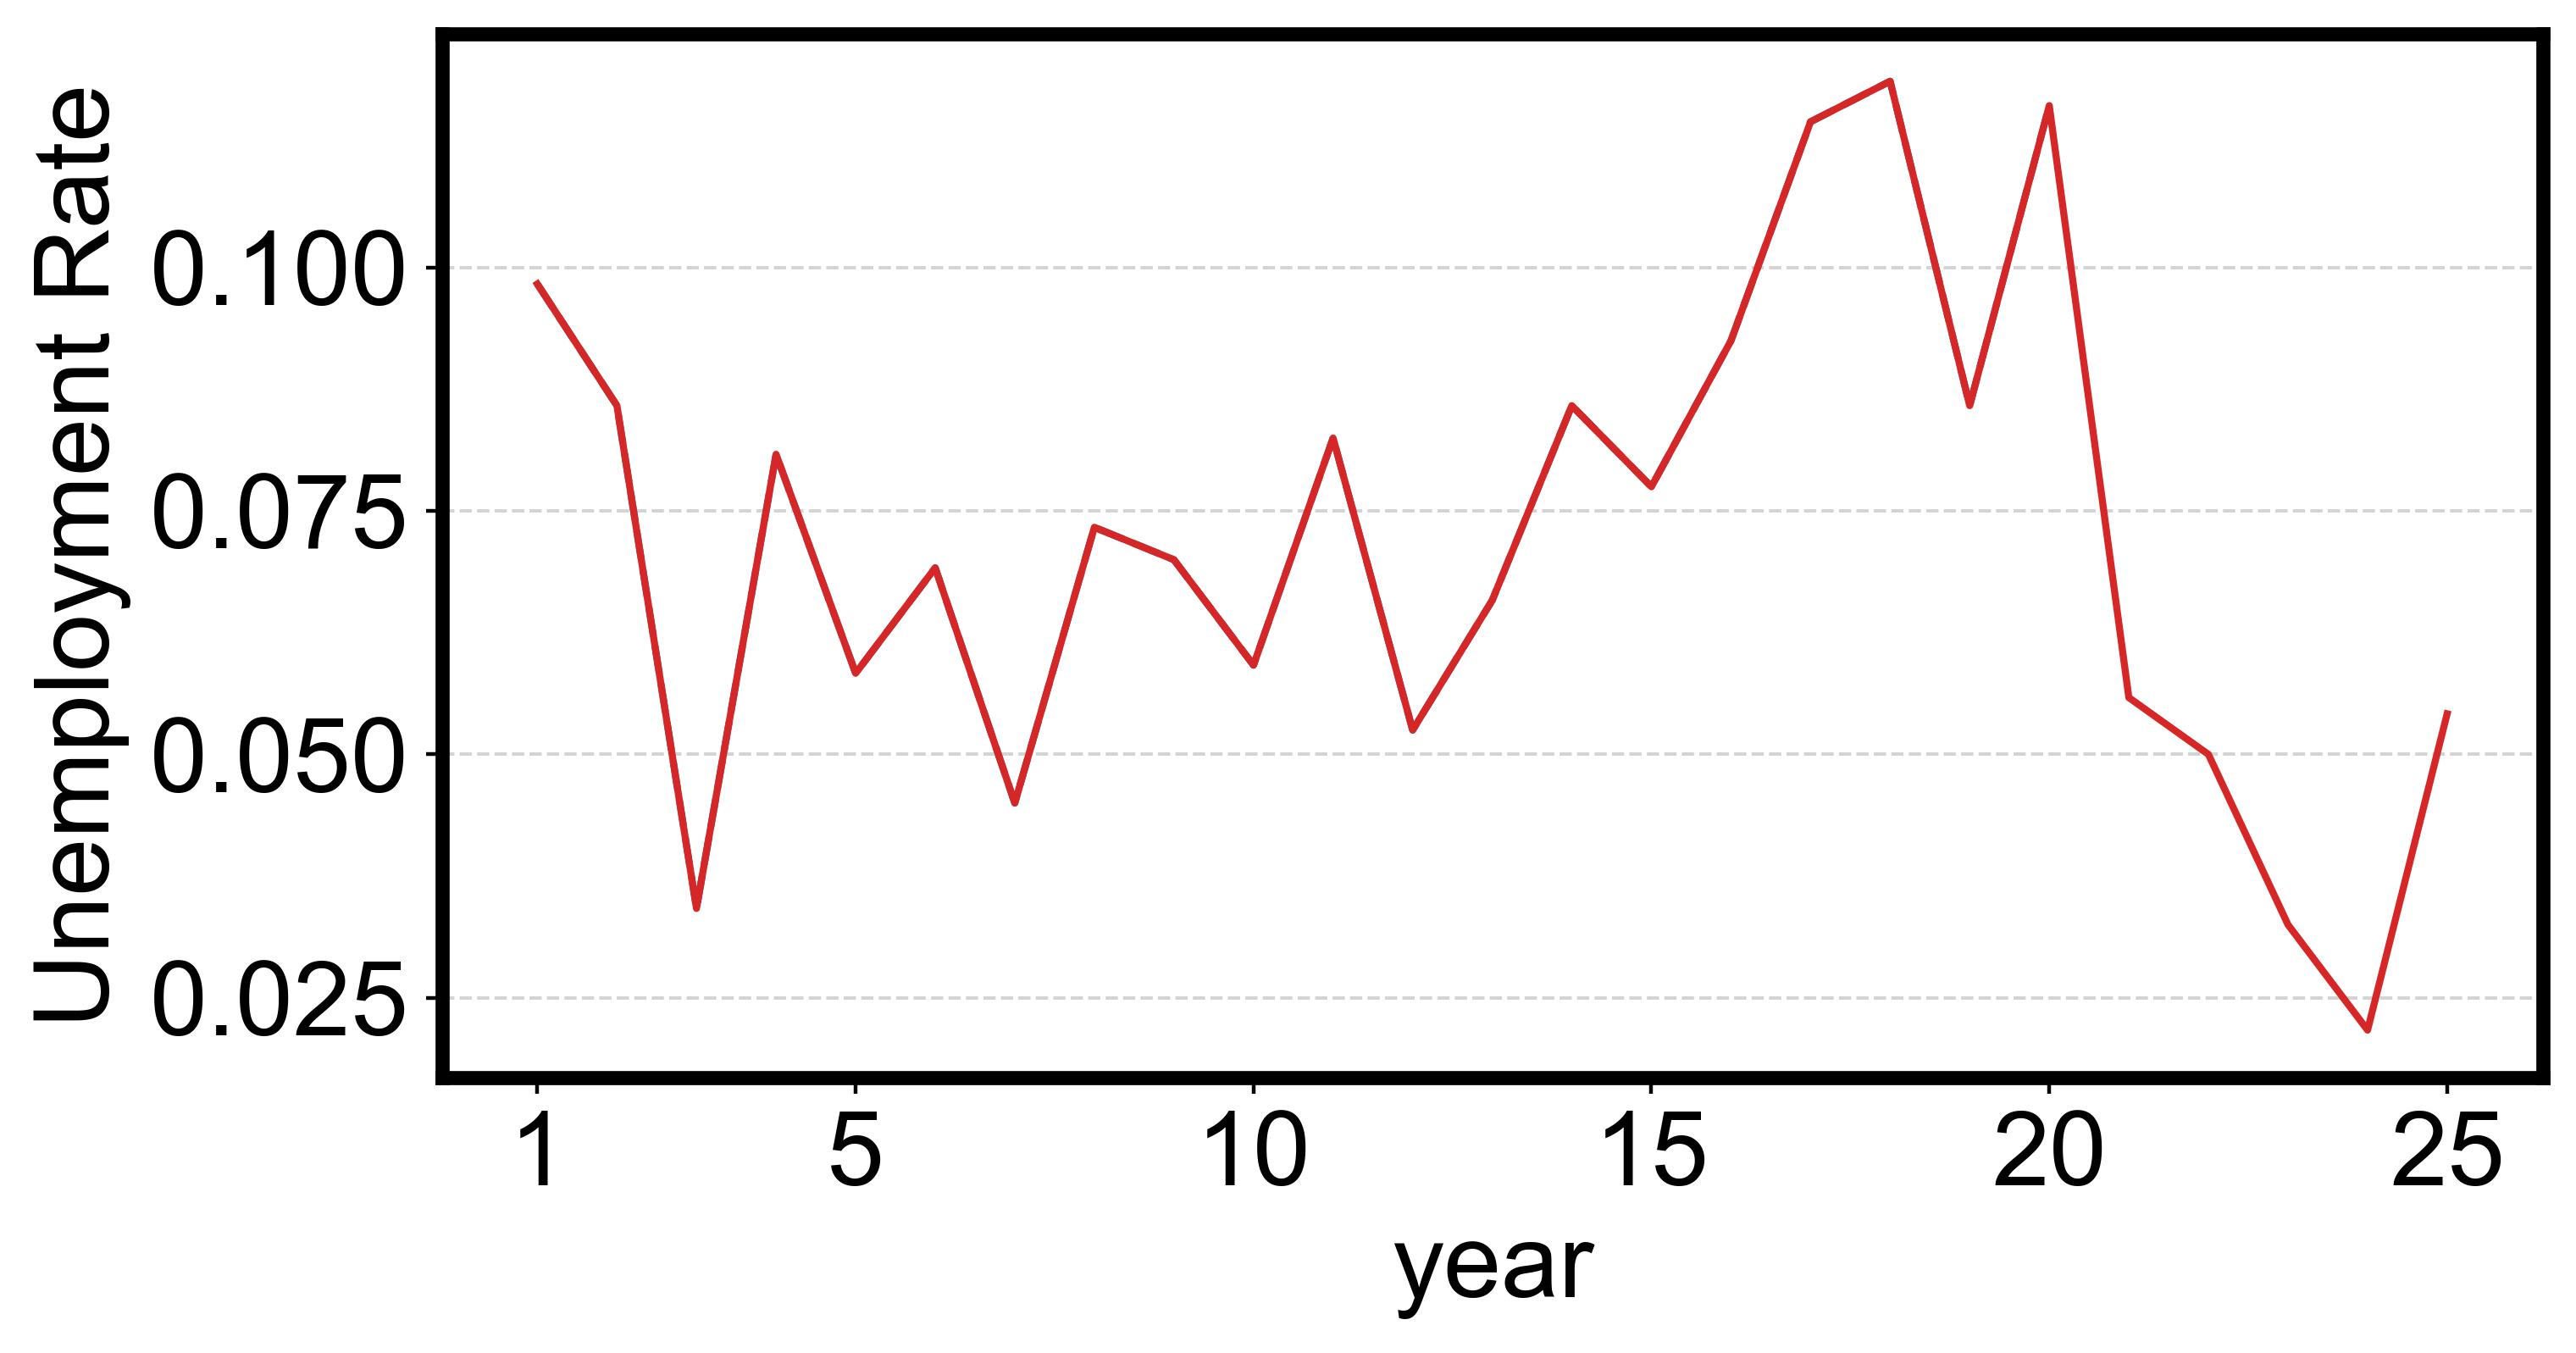
\includegraphics[width=0.9\linewidth]{figs/unemployment-year-continue.jpg} \
\caption{Unemployment rate for 25 years.}\label{fig::unemployment-c}
\end{figure}

\paragraph{Sensitivity and Robustness} We increase the number to 300 and run the simulation again. Figure \ref{fig::sensitivity} shows consistently stable and plausible inflation rates similar to those of 100 agents, which holds for other indicators as well. Therefore, the simulation results are insensitive to the number of agents.

\begin{figure}[h!]
\centering
{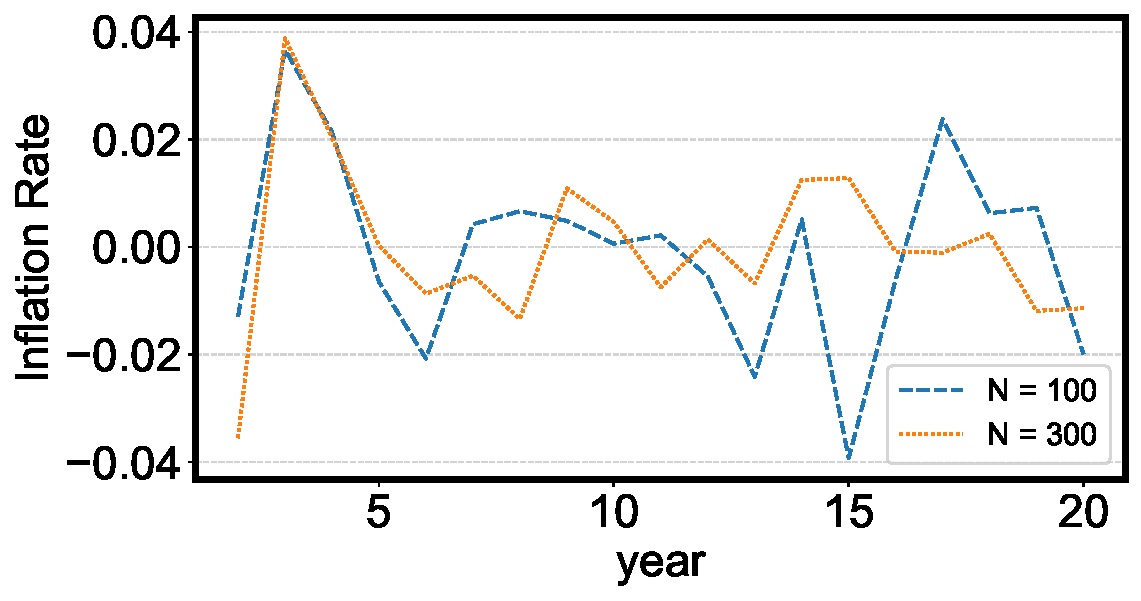
\includegraphics[width=0.9\linewidth]{figs/inflation-year-N.pdf}}
\caption{Inflation rate under different number of agents.}\label{fig::sensitivity}
\end{figure}

We conduct five simulations for each agent model and present the inflation rate in Figure \ref{fig::robustness}. It is evident that the simulations based on EconAgent are robust and consistently yield more stable and plausible results, which is also true for other indicators. Importantly, there are no significant differences in terms of stability and numerical scale among the simulations.

\begin{figure}[h!]
\centering
\subfloat{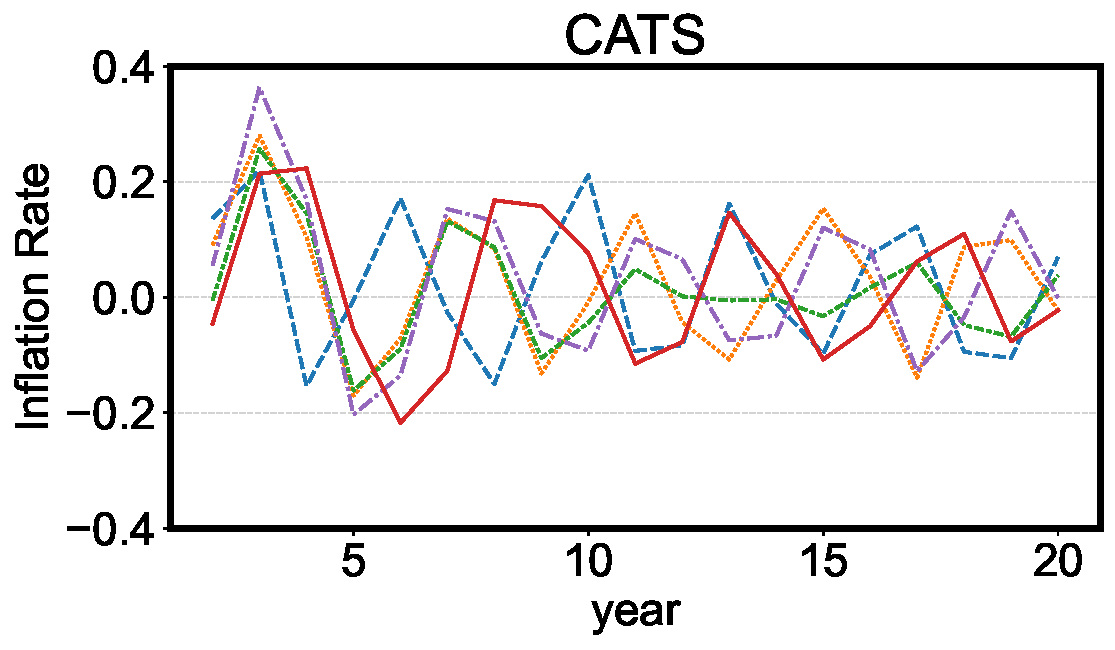
\includegraphics[width=0.9\linewidth]{figs/inflation-year-multi-run-CATS.pdf}} \
\subfloat{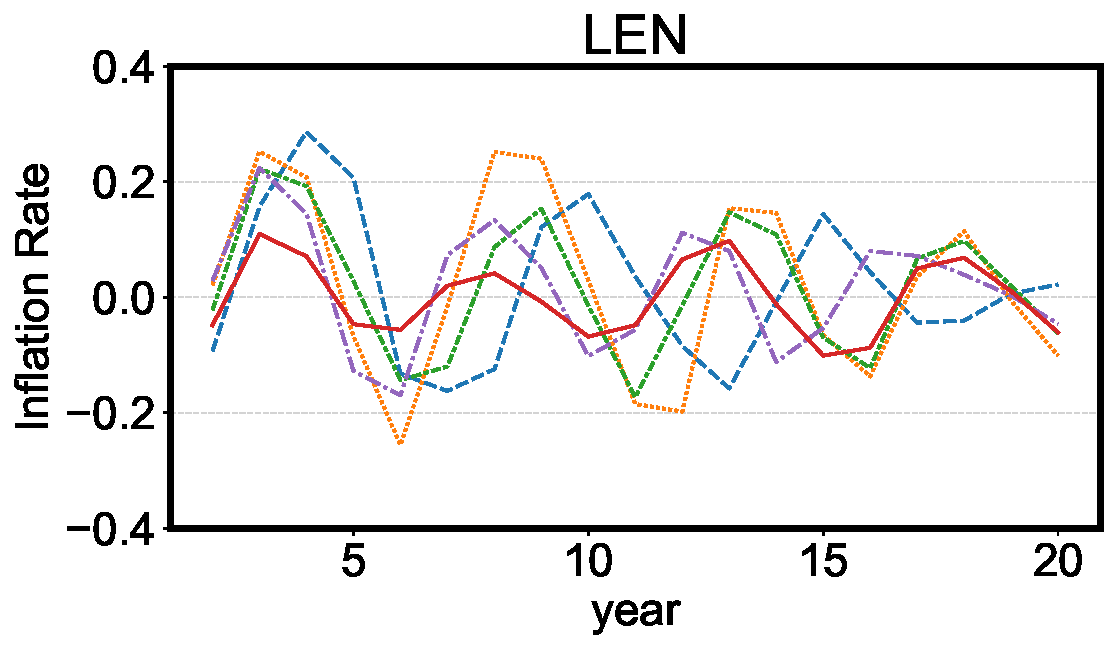
\includegraphics[width=0.9\linewidth]{figs/inflation-year-multi-run-LEN.pdf}} \
\subfloat{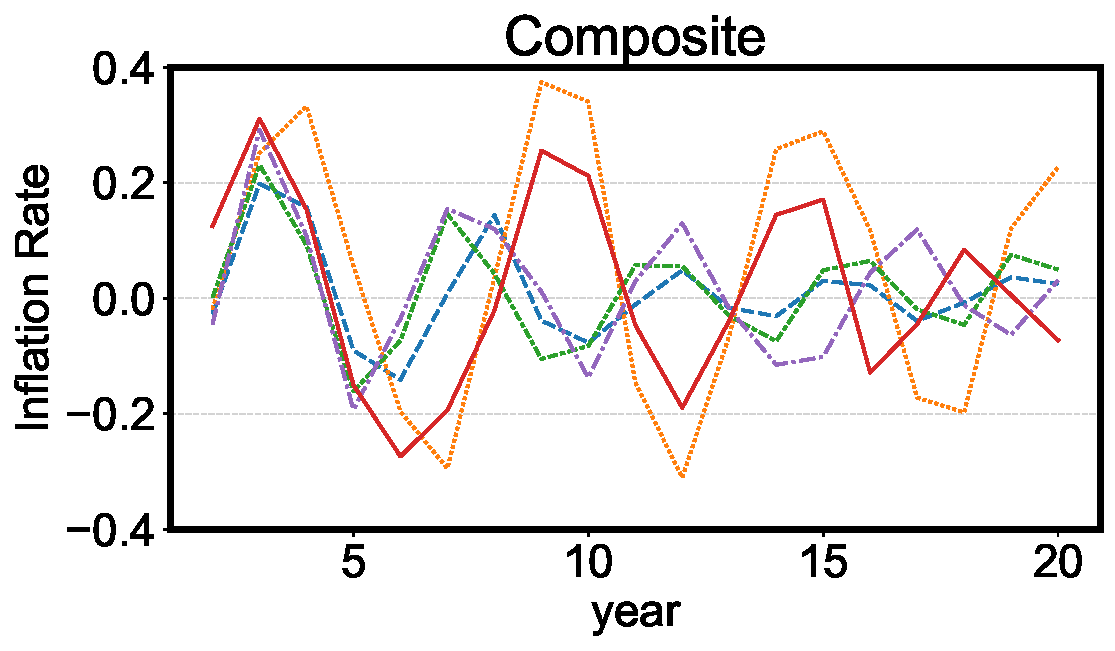
\includegraphics[width=0.9\linewidth]{figs/inflation-year-multi-run-Composite.pdf}} \
\subfloat{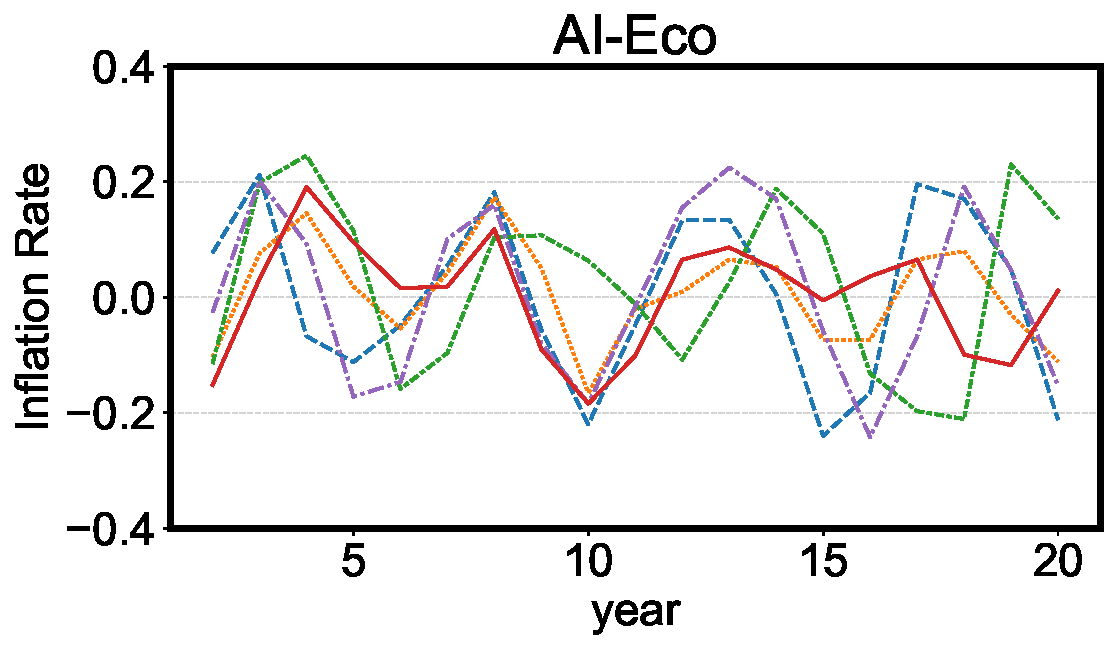
\includegraphics[width=0.9\linewidth]{figs/inflation-year-multi-run-AI-Eco.pdf}} \
\subfloat{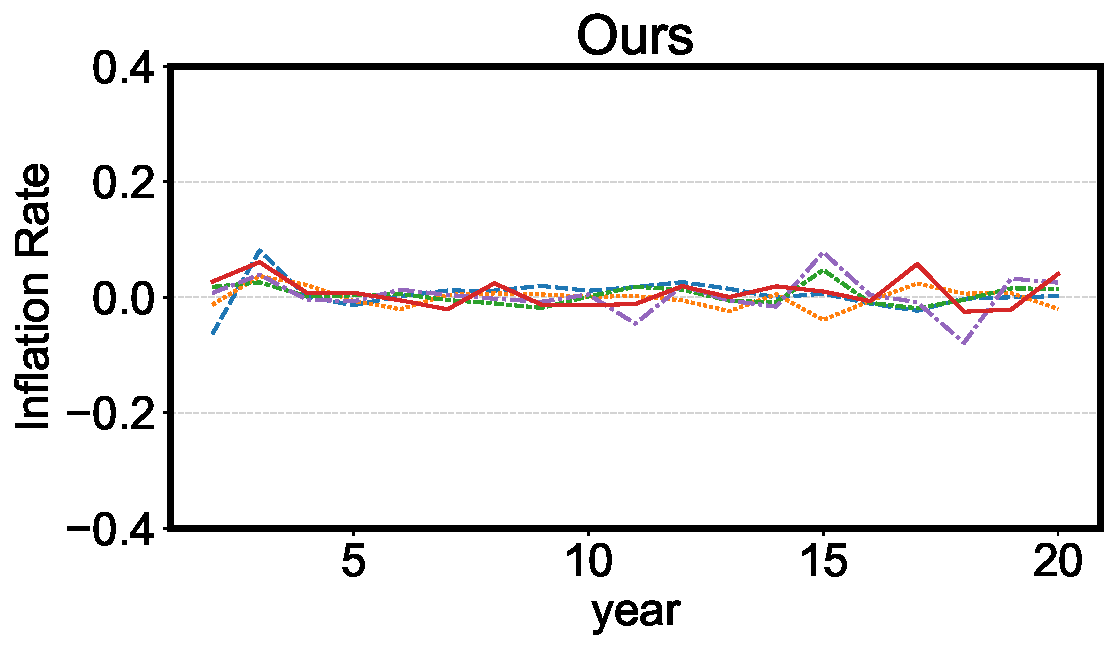
\includegraphics[width=0.9\linewidth]{figs/inflation-year-multi-run-Ours.pdf}} \
\caption{Simulation variance across five experiments for different agent models.}\label{fig::robustness}
\end{figure}